% Chapter Template

\chapter{Conclusiones} % Main chapter title

\label{Chapter5} % Change X to a consecutive number; for referencing this chapter elsewhere, use \ref{ChapterX}


%----------------------------------------------------------------------------------------

En este capítulo se destacan los objetivos cumplidos con el trabajo realizado y se plantea el camino a seguir para realizar mejoras futuras.

%----------------------------------------------------------------------------------------
%	SECTION 1
%----------------------------------------------------------------------------------------

\section{Resultados obtenidos }

Los objetivos y requerimientos planteados al inicio del proyecto fueron cumplidos en su totalidad. El tiempo de ejecución de las tareas fue similar al estimado, pero no pudo respetarse el cronograma mostrado en la figura \ref{fig:diagramaGantt}. Esto se debe a la manifestación de algunos de los riesgos identificados en la planificación. En primer lugar se manifestó la imposibilidad de disponer del electrodo de pH en tiempo y forma, por lo que la tarea 5.1 se atrasó hasta junio. Además, las tareas 6.2 y 6.3 se vieron afectadas por la ocurrencia del riesgo asociado a la imposibilidad de acceder al laboratorio a causa del aislamiento. A pesar de la ocurrencia de estos riesgos, el único efecto fue el cambio de los plazos planificados y las tareas fueron ejecutadas a la normalidad en el tiempo estimado.

Por último, es importante destacar el uso de los conocimientos y técnicas utilizadas en el desarrollo y que fueron adquiridas durante el cursado de la especialización:
\begin{itemize}
 \item El uso de máquinas de estado en la interfaz de usuario.
 \item El uso de FreeRTOS para la ejecución de diferentes tareas.
 \item El uso de protocolos y comunicaciones, como ser UART, SPI y Wi-Fi.
 \item El uso de técnicas de diseño de esquemáticos y circuitos impresos.
\end{itemize}

Gracias a los aportes al desarrollo mediante los trabajos prácticos realizados en las asignaturas correspondientes, se logró integrar conceptos y cumplir los plazos planificados para estas instancias.

%La idea de esta sección es resaltar cuáles son los principales aportes del trabajo realizado y cómo se podría continuar. Debe ser especialmente breve y concisa. Es buena idea usar un listado para enumerar los logros obtenidos.
%
%Algunas preguntas que pueden servir para completar este capítulo:
%
%\begin{itemize}
%\item ¿Cuál es el grado de cumplimiento de los requerimientos?
%\item ¿Cuán fielmente se puedo seguir la planificación original (cronograma incluido)?
%\item ¿Se manifestó algunos de los riesgos identificados en la planificación? ¿Fue efectivo el plan de mitigación? ¿Se debió aplicar alguna otra acción no contemplada previamente?
%\item Si se debieron hacer modificaciones a lo planificado ¿Cuáles fueron las causas y los efectos?
%\item ¿Qué técnicas resultaron útiles para el desarrollo del proyecto y cuáles no tanto?
%\end{itemize}


%----------------------------------------------------------------------------------------
%	SECTION 2
%----------------------------------------------------------------------------------------
\section{Trabajo futuro}

El siguiente paso a seguir es realizar mejoras funcionales respecto al \textit{firmware}. Hay detalles a mejorar en la interfaz de usuario, por ejemplo la gráfica del pH respecto al tiempo debería ser de pH respecto al volumen. Además, se piensa agregar una opción para que el usuario pueda configurar la red Wi-Fi a la cual desea conectar el dispositivo. 

Las principales mejoras respecto al hardware dependen de la inclusión de nuevos componentes. La utilización de un sensor de temperatura permitiría ajustar el valor de pH para cuando se trabaje con muestras que no estén a temperatura ambiente. Además, el uso de un sensor de flujo permitiría tener una medida del volumen inyectado y crear un sistema de control de lazo cerrado.


\begin{landscape}
	\begin{figure}[p]
	\centering 
	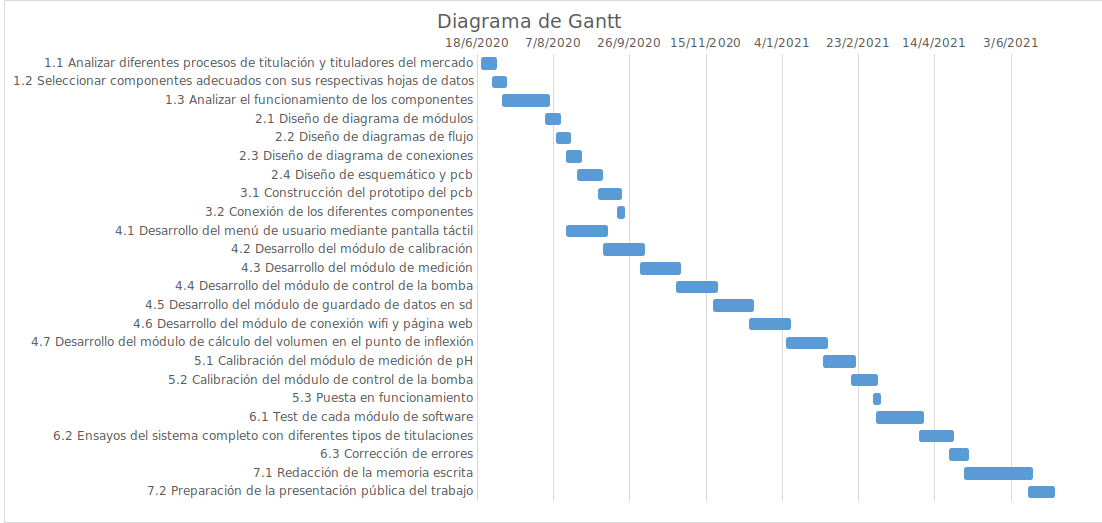
\includegraphics[width=1.5\textwidth]{./Figures/DiagramaGantt.png}
	\caption{Diagrama de Gantt: gráfico}
	\label{fig:diagramaGantt}
	\end{figure}
\end{landscape}
